% sections/04-framework.tex — conceptual centerpiece (approved CP2-lock state).
\section{The Autonomy $\times$ Loop Framework}
\label{sec:framework}

\subsection{Unit of Analysis}
Records are typed before classification: only \emph{systems}, \emph{clearly specified
experiments}, and \emph{incident documentations} receive autonomy levels; benchmarks carry
\emph{probed loop phases}; datasets carry task domains; surveys and systematizations carry the
\emph{documented systems} they describe. This prevents a paper about autonomous systems from
becoming an autonomous-system datapoint --- our corpus contains one such systematization of
AIxCC~\cite{r7sokaixcc2026}, and it is classified \emph{n/a} on both axes.

\subsection{Axis A: Decision Authority}
The autonomy gradient is operationalized by one question: \textbf{who chooses the next action?}
\emph{A0 assistive}: no acting system; a prompted model responds. \emph{A1
pipeline-orchestrated}: a fixed controller determines the workflow; the model fills stages.
Tool use does not imply A1$\rightarrow$A2 --- a system invoking ten tools under fixed control
remains A1. \emph{A2 task agent}: the model dynamically selects actions and tools within a
bounded task environment. \emph{A3 autonomous production hunter}: independent planning,
execution, validation, and reporting (\emph{all four verbs}) in environment class E2 ---
production or production-like external targets (E0=synthetic/benchmark; E1=realistic but
sandboxed or competition). Two corollaries do heavy lifting: \emph{no human interaction}
$\neq$ A3, since AIxCC CRSs satisfied execution autonomy inside forked challenge repositories;
and the \emph{weakest-missing-condition rule}: every autonomy claim is graded by its weakest
unmet condition, never by headline percentages --- which is how ``fully automated'' XBOW
classifies A2 (policy-mandated pre-submission review) and how the GTG-1002 incident remains
\emph{uncertain} rather than A3.

\subsection{Axis B: Loop Position}
B1 discovery; B2 triage/validation/exploitation; B3 patching/repair; B4
redeployment/regression/monitoring. Axis B is a set: multi-phase systems are recorded as sets
(e.g., AIxCC CRSs $\{B1,B2,B3\}$) and drawn with neutral connectors denoting documented
coverage, not inferred sequencing.

\subsection{The Map}
Figure~\ref{fig:abmap} places the in-window corpus; Table~\ref{tab:abmatrix} lists all 36
records individually. The A2 row is populated across all three loop phases; the A3 row is
empty under the operational definition; B4 exists only as loop-transition documentation tied to
documented systems. Counts are computed programmatically from per-record YAML evidence files.

% figures/autonomy-loop-map.tex — F2 v3 (layout-aligned revision)
% Unit of analysis and evidence classifications are unchanged; only visual layout/alignment is revised.
\begin{figure*}[t]
\centering
\resizebox{\textwidth}{!}{%
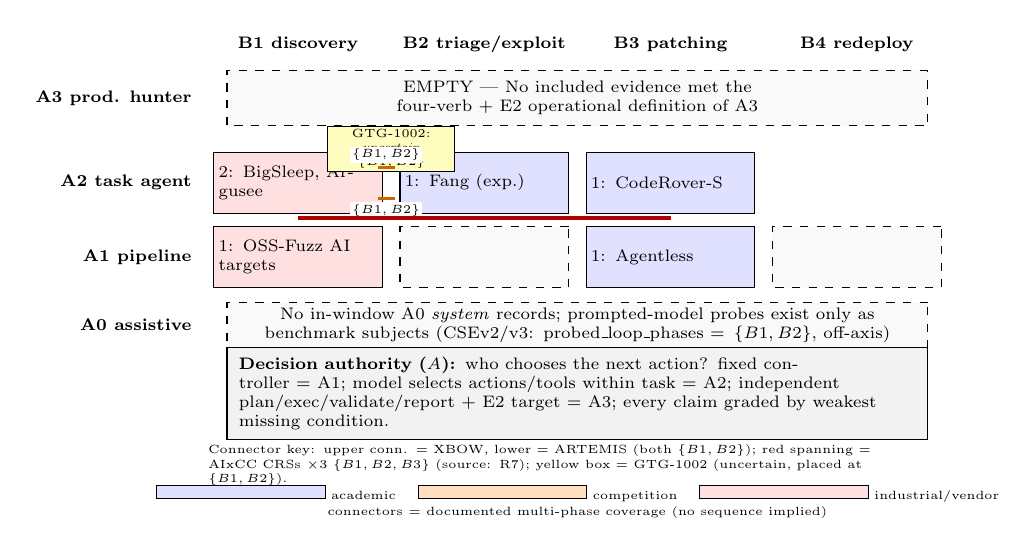
\begin{tikzpicture}[
  cell/.style={draw,align=left,font=\scriptsize,text width=2.35cm,minimum height=0.90cm,inner sep=2pt},
  acad/.style={cell,fill=blue!12}, comp/.style={cell,fill=orange!25},
  ind/.style={cell,fill=red!12}, empt/.style={cell,dashed,fill=gray!5},
  ctx/.style={draw,fill=gray!10,font=\scriptsize,align=left,text width=10.0cm,inner sep=4pt},
  lab/.style={font=\scriptsize\bfseries},
  conn/.style={-,very thick,orange!80!black},
  scale=0.86,transform shape]

% Phase headers: one shared grid.
\node[lab] at (0.0,4.30) {B1 discovery};
\node[lab] at (2.75,4.30) {B2 triage/exploit};
\node[lab] at (5.5,4.30) {B3 patching};
\node[lab] at (8.25,4.30) {B4 redeploy};

% Autonomy labels.
\node[lab,anchor=east] at (-1.45,3.50) {A3 prod. hunter};
\node[lab,anchor=east] at (-1.45,2.25) {A2 task agent};
\node[lab,anchor=east] at (-1.45,1.15) {A1 pipeline};
\node[lab,anchor=east] at (-1.45,0.15) {A0 assistive};

% A3 row.
\node[empt,minimum width=10.35cm,minimum height=0.82cm,text width=10.0cm,align=center] at (4.125,3.50)
 {\scriptsize EMPTY --- No included evidence met the four-verb $+$ E2 operational definition of A3};

% A2 row.
\node[ind]  at (0.0,2.25) {2: BigSleep, Argusee};
\node[acad] at (2.75,2.25) {1: Fang (exp.)};
\node[acad] at (5.5,2.25) {1: CodeRover-S};
% GTG-1002: narrow yellow label in B1--B2 gutter (its loop phases).
\node[font=\tiny,anchor=center,draw,fill=yellow!25,align=center,text width=1.8cm,minimum height=0.55cm,inner sep=1pt]
  at (1.375,2.75) {GTG-1002: \emph{uncertain} $\{B1,B2\}$};

% Neutral documented-coverage connectors.  The line itself stays entirely in the gutter;
% the phase-set labels sit in the whitespace immediately adjacent to that gutter.
\draw[conn] (1.175,2.48) -- (1.425,2.48);
\node[font=\tiny,anchor=south,fill=white,inner sep=1pt] at (1.30,2.53) {$\{B1,B2\}$};
\draw[conn] (1.175,2.02) -- (1.425,2.02);
\node[font=\tiny,anchor=north,fill=white,inner sep=1pt] at (1.30,1.97) {$\{B1,B2\}$};
% AIxCC is a documented B1--B3 multi-phase record; red connector spans B1--B3.
\draw[conn,red!70!black] (0.0,1.73) -- (5.5,1.73);


% A1 row.
\node[ind]  at (0.0,1.15) {1: OSS-Fuzz AI targets};
\node[empt] at (2.75,1.15) {};
\node[acad] at (5.5,1.15) {1: Agentless};
\node[empt] at (8.25,1.15) {};

% A0 note, kept inside the same B-grid.
\node[empt,minimum width=10.35cm,minimum height=0.62cm,text width=10.0cm,align=center] at (4.125,0.15)
 {\scriptsize No in-window A0 \emph{system} records; prompted-model probes exist only as benchmark
  subjects (CSEv2/v3: probed\_loop\_phases $=\{B1,B2\}$, off-axis)};

% Compact annotation band.
\node[ctx,minimum width=10.35cm] at (4.125,-0.86)
 {\textbf{Decision authority ($A$):} who chooses the next action? fixed controller $=$ A1;
  model selects actions/tools within task $=$ A2; independent plan/exec/validate/report $+$ E2 target $=$ A3;
  every claim graded by weakest missing condition.};

\node[font=\tiny,anchor=west,text width=10.35cm] at (-1.45,-1.92)
 {Connector key: upper conn. $=$ XBOW, lower $=$ ARTEMIS (both $\{B1,B2\}$); red spanning $=$ AIxCC CRSs $\times$3 $\{B1,B2,B3\}$ (source: R7); yellow box $=$ GTG-1002 (uncertain, placed at $\{B1,B2\}$).};

\node[font=\tiny,align=center] at (4.125,-2.34)
 {\tikz{\node[acad,minimum size=2mm]{};} academic \quad
  \tikz{\node[comp,minimum size=2mm]{};} competition \quad
  \tikz{\node[ind,minimum size=2mm]{};} industrial/vendor};
\node[font=\tiny,align=center] at (4.125,-2.62)
 {connectors $=$ documented multi-phase coverage (no sequence implied)};
\end{tikzpicture}
}
\caption{Autonomy $\times$ loop map over autonomy-bearing records (in-window corpus). Only
records whose unit is a system, a clearly specified experiment, or an incident documentation
receive $A$-levels (12 records, plus 2 general-SE comparators); benchmarks report \emph{probed loop phases},
datasets report \emph{task domains}, and systematization papers report \emph{documented systems}. Axis B is the
set $\{B1..B4\}$; multi-phase operation uses neutral connectors denoting documented coverage.
The A3 row is empty under the four-verb $+$ E2-environment definition; the nearest candidate
(GTG-1002) remains uncertain under the weakest-missing-condition rule.}
\label{fig:abmap}
\end{figure*}


\subsection{Migration, 2024 $\rightarrow$ June 2026}
Early in-window records are dominated by benchmarked/prompted capability evaluation, while the
system-bearing evidence shifts toward A1 pipeline automation (OSS-Fuzz's LLM stages; Agentless)
and A2 task agents --- arriving first as seeded production research (Big Sleep, November 2024),
then proliferating across independent industrial (Argusee, May 2025; XBOW, June 2025),
competition (AIxCC finals, August 2025), and production-network experimental settings (ARTEMIS).
We emphasize what this phrasing avoids: our corpus contains no in-window A0 systems, so claims
of a field-wide ``A0$\rightarrow$A1$\rightarrow$A2 migration'' would outrun the evidence; what
migrated is where humans sit (boundaries: seeds, entry points, review, reporting) and what gets
scored. The 2026 record adds consolidation --- four systematizations, an infrastructure-risk
cluster around agent tool protocols, and the first institutionalized B4 documentation.

% tables/autonomy-loop-matrix.tex — v4 (CP4 blocker fix): body REGENERATED from the frozen
% CP2-lock schema (14 autonomy-bearing / 2 background / 2 loop-transition-doc / 18 context).
% Root cause of prior staleness: v3 header comment updated while tabular body stayed v2.
% Source of truth: evidence/autonomy-loop-assignments.csv + corpus/included/*.yaml.
\begin{table*}[t]
\centering
\caption{Complete record-level classification (36 records). $A$ = autonomy level;
$B$ = loop-position set; T = temporal scope. Only systems, clearly specified experiments, and
incident documentation bear $A$-levels; benchmarks report probed phases ($^{p}$); datasets
report task domains; systematizations are n/a with documented systems. Per-record behavioral
evidence: \texttt{evidence/autonomy-loop-assignments.csv}.}
\label{tab:abmatrix}
\scriptsize
\setlength{\tabcolsep}{3.0pt}
\resizebox{\textwidth}{!}{%
\begin{tabular}{lllll}
\hline
Record & Year & T & $A$ & $B$-set / role \\
\hline
\multicolumn{5}{l}{\emph{(i) In-window autonomy-bearing records (14)}}\\
bigsleep2024naptime      & 2024 & in & A2        & $\{B1\}$ \\
argusee2025              & 2025 & in & A2        & $\{B1\}$ \\
fang2024one-day          & 2024 & in & A2 (exp.) & $\{B2\}$ \\
sweagent2024             & 2024 & in & A2        & $\{B3\}$ \\
autocoderoever2024       & 2024 & in & A2        & $\{B3\}$ \\
ossfuzz-aifixing2024     & 2024 & in & A2        & $\{B3\}$ \\
xbow2025                 & 2025 & in & A2        & $\{B1{+}B2\}$ \\
artemis2025comparing     & 2025 & in & A2 (exp.) & $\{B1{+}B2\}$ \\
r7-CRS-cluster recs:     &      &    &           &              \\
\quad tob-buttercup2025  & 2025 & in & A2        & $\{B1{+}B2{+}B3\}$ \\
\quad teamatlanta-sqlite2024 & 2024 & in & A2    & $\{B1{+}B2{+}B3\}$ \\
\quad teamatlanta-afc2025    & 2025 & in & A2    & $\{B1{+}B2{+}B3\}$ \\
gtg1002-2025             & 2025 & in & uncertain & $\{B1{+}B2\}$ \\
ossfuzz-levelingup2024   & 2024 & in & A1        & $\{B1\}$ \\
agentless2024            & 2024 & in & A1        & $\{B3\}$ \\
\hline
\multicolumn{5}{l}{\emph{(ii) Background anchors --- excluded from primary counts (2)}}\\
intercode2023            & 2023 & bg & A1        & $\{B2\}$ \\
csev12023                & 2023 & bg & A0        & $\{B1\}$ \\
\hline
\multicolumn{5}{l}{\emph{(iii) Loop-transition documentation --- B4 tied to systems (2)}}\\
openssfretro2026         & 2026 & in & (A2 CRS cluster) & documents $B3{\to}B4$ \\
bloggoogle-summer2025    & 2025 & in & (A2 BigSleep)    & documents $B1{\to}B4$ redeploy \\
\hline
\multicolumn{5}{l}{\emph{(iv) Off-axis / context records (18)}}\\
cybench2024              & 2024 & in & n/a & benchmark; probed $\{B2\}^p$; embedded A2-class scaffold \\
nyuctfbench2024          & 2024 & in & n/a & benchmark; probed $\{B2\}^p$; embedded A2-class scaffold \\
csev22024                & 2024 & in & n/a & benchmark; probed $\{B1,B2\}^p$ \\
csev32024                & 2024 & in & n/a & benchmark; probed $\{B1,B2\}^p$ \\
primevul2024             & 2024 & in & n/a & dataset; task domain $B1$ detection \\
rissebohme2024           & 2024 & in & n/a & methodological critique \\
mcpeco2025               & 2025 & in & n/a & MCP ecosystem measurement \\
mcpgov2025               & 2025 & in & n/a & MCP governance \\
mcpspec2026              & 2026 & in & n/a & MCP spec analysis \\
mcppoison2026            & 2026 & in & n/a & MCP tool poisoning \\
nvdcve20256965           & 2025 & in & n/a & registry record (CVE-2025-6965) \\
zhang2024when (R1)       & 2024 & in & n/a & survey (SLR) \\
r2slr2024remediation(R2) & 2024 & in & n/a & survey (SLR) \\
sheng2025csur (R4)       & 2025 & in & n/a & survey (paywalled; metadata) \\
r5usenix26agentic (R5)   & 2026 & in & n/a & survey (agentic-AI security) \\
tosemslr2026 (R6)        & 2026 & in & n/a & survey (263 studies; repo open) \\
r7sokaixcc2026 (R7)      & 2026 & in & n/a & survey(systematization); documents Atlantis, Buttercup,\\
                         &      &    &     & Theori-SRS, RoboDuck, FuzzingBrain, Lacrosse, Shellphish \\
r3survey2026pentest (R3) & 2026 & OUT& n/a & survey comparator (out-of-window) \\
\hline
\multicolumn{5}{l}{\scriptsize Totals: 14 autonomy-bearing ($A1{\times}2$, $A2{\times}11$, uncertain${\times}1$, $A3{=}0$)
$+$ 2 background $+$ 2 loop-transition $+$ 18 context $=$ 36 records.}\\
\end{tabular}
}
\end{table*}

